% ch4-laser

\chapter [Laser-Based IMS]{Laser-Based Intersection Management System}

In this chapter is described the development of a laser based system for intersection monitoring

\section{Preprocessing and Background removal}

The first step in processing laser data is the removal of irrelevant frames, maybe due to communication errors or due to corrupted data. For this stage is proposed a filter based on the of entropy of data, calculated for each frame, because it is not expected to have sudden changes in entropy between consecutive frames. 

\begin{figure}[ht!]
\centering
% Title: glps_renderer figure
% Creator: GL2PS 1.3.8, (C) 1999-2012 C. Geuzaine
% For: Octave
% CreationDate: Fri Jun 12 09:55:58 2015
\setlength{\unitlength}{1pt}
\begin{picture}(0,0)
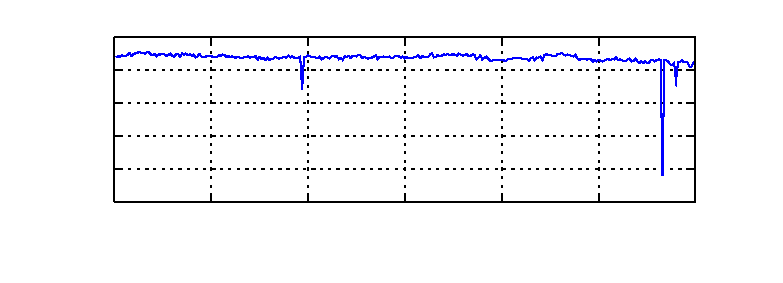
\includegraphics{fig/4/entropy_frame-inc}
\end{picture}%
\begin{picture}(360,120)(0,0)
\fontsize{10}{0}
\selectfont\put(46.8,25.9892){\makebox(0,0)[t]{\textcolor[rgb]{0,0,0}{{0}}}}
\fontsize{10}{0}
\selectfont\put(93.3,25.9892){\makebox(0,0)[t]{\textcolor[rgb]{0,0,0}{{50}}}}
\fontsize{10}{0}
\selectfont\put(139.8,25.9892){\makebox(0,0)[t]{\textcolor[rgb]{0,0,0}{{100}}}}
\fontsize{10}{0}
\selectfont\put(186.3,25.9892){\makebox(0,0)[t]{\textcolor[rgb]{0,0,0}{{150}}}}
\fontsize{10}{0}
\selectfont\put(232.8,25.9892){\makebox(0,0)[t]{\textcolor[rgb]{0,0,0}{{200}}}}
\fontsize{10}{0}
\selectfont\put(279.3,25.9892){\makebox(0,0)[t]{\textcolor[rgb]{0,0,0}{{250}}}}
\fontsize{10}{0}
\selectfont\put(325.8,25.9892){\makebox(0,0)[t]{\textcolor[rgb]{0,0,0}{{300}}}}
\fontsize{10}{0}
\selectfont\put(41.8,30.9898){\makebox(0,0)[r]{\textcolor[rgb]{0,0,0}{{0}}}}
\fontsize{10}{0}
\selectfont\put(41.8,46.7918){\makebox(0,0)[r]{\textcolor[rgb]{0,0,0}{{1}}}}
\fontsize{10}{0}
\selectfont\put(41.8,62.5939){\makebox(0,0)[r]{\textcolor[rgb]{0,0,0}{{2}}}}
\fontsize{10}{0}
\selectfont\put(41.8,78.3959){\makebox(0,0)[r]{\textcolor[rgb]{0,0,0}{{3}}}}
\fontsize{10}{0}
\selectfont\put(41.8,94.198){\makebox(0,0)[r]{\textcolor[rgb]{0,0,0}{{4}}}}
\fontsize{10}{0}
\selectfont\put(41.8,110){\makebox(0,0)[r]{\textcolor[rgb]{0,0,0}{{5}}}}
\fontsize{10}{0}
\selectfont\put(186.3,12.9892){\makebox(0,0)[t]{\textcolor[rgb]{0,0,0}{{Frame}}}}
\fontsize{10}{0}
\selectfont\put(31.8,70.4949){\rotatebox{90}{\makebox(0,0)[b]{\textcolor[rgb]{0,0,0}{{Entropy}}}}}
\end{picture}

\caption{Entropy of frames 1 to 300 of laser readings from sensor 7.}
\label{entropy_frames}
\end{figure}

In this case histogram-based entropy estimation is used, which is commonly used in image processing. The first step is to compute histogram $P$ of the frame $f$ using 256 bins, then $P$ is normalized using the sum of each bin value. After this, entropy $H$ of frame $f$ is calculated as follows:

\begin{equation}
 H(P)=-\sum_{i=0}^{255}{ p_i.\log_{2}{p_i}} 
\end{equation}

In figure \ref{entropy_frames} is depicted the evolution of entropy calculated on 300 frames of a laser reading. It can be seen that there are frames with abrupt changes in entropy value, for example frames 97 and 283.


Figure \ref{l7-f283} shows the actual laser data of frame 283 and its neighbours and also entropy values aroud objective frame. It is clear now that frame 283 is inconsistent with frames 282 and 284, for this reason this frame is considered as corrupted and should be discarded for next stages

\begin{figure}[ht!]
\centering
% Title: glps_renderer figure
% Creator: GL2PS 1.3.8, (C) 1999-2012 C. Geuzaine
% For: Octave
% CreationDate: Fri Jun 12 10:16:39 2015
\setlength{\unitlength}{1pt}
\begin{picture}(0,0)
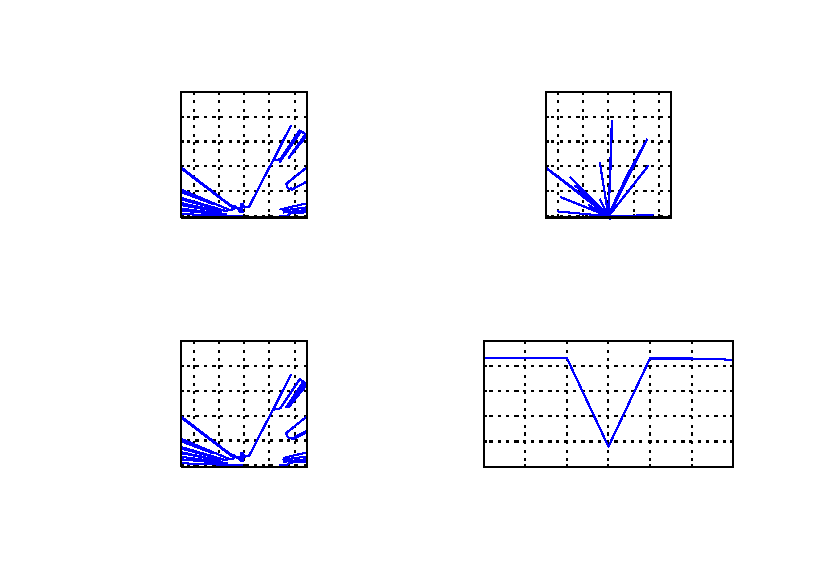
\includegraphics{fig/4/l7-f283-inc}
\end{picture}%
\begin{picture}(380,260)(0,0)
\fontsize{10}{0}
\selectfont\put(85.089,158.564){\makebox(0,0)[t]{\textcolor[rgb]{0,0,0}{{-40}}}}
\fontsize{10}{0}
\selectfont\put(97.1695,158.564){\makebox(0,0)[t]{\textcolor[rgb]{0,0,0}{{-20}}}}
\fontsize{10}{0}
\selectfont\put(109.25,158.564){\makebox(0,0)[t]{\textcolor[rgb]{0,0,0}{{0}}}}
\fontsize{10}{0}
\selectfont\put(121.33,158.564){\makebox(0,0)[t]{\textcolor[rgb]{0,0,0}{{20}}}}
\fontsize{10}{0}
\selectfont\put(133.411,158.564){\makebox(0,0)[t]{\textcolor[rgb]{0,0,0}{{40}}}}
\fontsize{10}{0}
\selectfont\put(74.0152,164.196){\makebox(0,0)[r]{\textcolor[rgb]{0,0,0}{{0}}}}
\fontsize{10}{0}
\selectfont\put(74.0152,176.156){\makebox(0,0)[r]{\textcolor[rgb]{0,0,0}{{20}}}}
\fontsize{10}{0}
\selectfont\put(74.0152,188.117){\makebox(0,0)[r]{\textcolor[rgb]{0,0,0}{{40}}}}
\fontsize{10}{0}
\selectfont\put(74.0152,200.078){\makebox(0,0)[r]{\textcolor[rgb]{0,0,0}{{60}}}}
\fontsize{10}{0}
\selectfont\put(74.0152,212.039){\makebox(0,0)[r]{\textcolor[rgb]{0,0,0}{{80}}}}
\fontsize{10}{0}
\selectfont\put(74.0152,224){\makebox(0,0)[r]{\textcolor[rgb]{0,0,0}{{100}}}}
\fontsize{10}{0}
\selectfont\put(109.25,145.564){\makebox(0,0)[t]{\textcolor[rgb]{0,0,0}{{x [m]}}}}
\fontsize{10}{0}
\selectfont\put(52.0152,193.799){\rotatebox{90}{\makebox(0,0)[b]{\textcolor[rgb]{0,0,0}{{y [m]}}}}}
\fontsize{10}{0}
\selectfont\put(109.25,234){\makebox(0,0)[b]{\textcolor[rgb]{0,0,0}{{Frame 282}}}}
\fontsize{10}{0}
\selectfont\put(259.889,158.564){\makebox(0,0)[t]{\textcolor[rgb]{0,0,0}{{-40}}}}
\fontsize{10}{0}
\selectfont\put(271.97,158.564){\makebox(0,0)[t]{\textcolor[rgb]{0,0,0}{{-20}}}}
\fontsize{10}{0}
\selectfont\put(284.05,158.564){\makebox(0,0)[t]{\textcolor[rgb]{0,0,0}{{0}}}}
\fontsize{10}{0}
\selectfont\put(296.13,158.564){\makebox(0,0)[t]{\textcolor[rgb]{0,0,0}{{20}}}}
\fontsize{10}{0}
\selectfont\put(308.211,158.564){\makebox(0,0)[t]{\textcolor[rgb]{0,0,0}{{40}}}}
\fontsize{10}{0}
\selectfont\put(248.815,164.196){\makebox(0,0)[r]{\textcolor[rgb]{0,0,0}{{0}}}}
\fontsize{10}{0}
\selectfont\put(248.815,176.156){\makebox(0,0)[r]{\textcolor[rgb]{0,0,0}{{20}}}}
\fontsize{10}{0}
\selectfont\put(248.815,188.117){\makebox(0,0)[r]{\textcolor[rgb]{0,0,0}{{40}}}}
\fontsize{10}{0}
\selectfont\put(248.815,200.078){\makebox(0,0)[r]{\textcolor[rgb]{0,0,0}{{60}}}}
\fontsize{10}{0}
\selectfont\put(248.815,212.039){\makebox(0,0)[r]{\textcolor[rgb]{0,0,0}{{80}}}}
\fontsize{10}{0}
\selectfont\put(248.815,224){\makebox(0,0)[r]{\textcolor[rgb]{0,0,0}{{100}}}}
\fontsize{10}{0}
\selectfont\put(284.05,145.564){\makebox(0,0)[t]{\textcolor[rgb]{0,0,0}{{x [m]}}}}
\fontsize{10}{0}
\selectfont\put(226.815,193.799){\rotatebox{90}{\makebox(0,0)[b]{\textcolor[rgb]{0,0,0}{{y [m]}}}}}
\fontsize{10}{0}
\selectfont\put(284.05,234){\makebox(0,0)[b]{\textcolor[rgb]{0,0,0}{{Frame 283}}}}
\fontsize{10}{0}
\selectfont\put(85.089,38.964){\makebox(0,0)[t]{\textcolor[rgb]{0,0,0}{{-40}}}}
\fontsize{10}{0}
\selectfont\put(97.1695,38.964){\makebox(0,0)[t]{\textcolor[rgb]{0,0,0}{{-20}}}}
\fontsize{10}{0}
\selectfont\put(109.25,38.964){\makebox(0,0)[t]{\textcolor[rgb]{0,0,0}{{0}}}}
\fontsize{10}{0}
\selectfont\put(121.33,38.964){\makebox(0,0)[t]{\textcolor[rgb]{0,0,0}{{20}}}}
\fontsize{10}{0}
\selectfont\put(133.411,38.964){\makebox(0,0)[t]{\textcolor[rgb]{0,0,0}{{40}}}}
\fontsize{10}{0}
\selectfont\put(74.0152,44.5956){\makebox(0,0)[r]{\textcolor[rgb]{0,0,0}{{0}}}}
\fontsize{10}{0}
\selectfont\put(74.0152,56.5565){\makebox(0,0)[r]{\textcolor[rgb]{0,0,0}{{20}}}}
\fontsize{10}{0}
\selectfont\put(74.0152,68.5173){\makebox(0,0)[r]{\textcolor[rgb]{0,0,0}{{40}}}}
\fontsize{10}{0}
\selectfont\put(74.0152,80.4782){\makebox(0,0)[r]{\textcolor[rgb]{0,0,0}{{60}}}}
\fontsize{10}{0}
\selectfont\put(74.0152,92.4391){\makebox(0,0)[r]{\textcolor[rgb]{0,0,0}{{80}}}}
\fontsize{10}{0}
\selectfont\put(74.0152,104.4){\makebox(0,0)[r]{\textcolor[rgb]{0,0,0}{{100}}}}
\fontsize{10}{0}
\selectfont\put(109.25,25.964){\makebox(0,0)[t]{\textcolor[rgb]{0,0,0}{{x [m]}}}}
\fontsize{10}{0}
\selectfont\put(52.0152,74.1988){\rotatebox{90}{\makebox(0,0)[b]{\textcolor[rgb]{0,0,0}{{y [m]}}}}}
\fontsize{10}{0}
\selectfont\put(109.25,114.4){\makebox(0,0)[b]{\textcolor[rgb]{0,0,0}{{Frame 284}}}}
\fontsize{10}{0}
\selectfont\put(224.2,38.964){\makebox(0,0)[t]{\textcolor[rgb]{0,0,0}{{280}}}}
\fontsize{10}{0}
\selectfont\put(244.15,38.964){\makebox(0,0)[t]{\textcolor[rgb]{0,0,0}{{281}}}}
\fontsize{10}{0}
\selectfont\put(264.1,38.964){\makebox(0,0)[t]{\textcolor[rgb]{0,0,0}{{282}}}}
\fontsize{10}{0}
\selectfont\put(284.05,38.964){\makebox(0,0)[t]{\textcolor[rgb]{0,0,0}{{283}}}}
\fontsize{10}{0}
\selectfont\put(304,38.964){\makebox(0,0)[t]{\textcolor[rgb]{0,0,0}{{284}}}}
\fontsize{10}{0}
\selectfont\put(323.95,38.964){\makebox(0,0)[t]{\textcolor[rgb]{0,0,0}{{285}}}}
\fontsize{10}{0}
\selectfont\put(343.9,38.964){\makebox(0,0)[t]{\textcolor[rgb]{0,0,0}{{286}}}}
\fontsize{10}{0}
\selectfont\put(219.212,43.9975){\makebox(0,0)[r]{\textcolor[rgb]{0,0,0}{{0}}}}
\fontsize{10}{0}
\selectfont\put(219.212,56.078){\makebox(0,0)[r]{\textcolor[rgb]{0,0,0}{{1}}}}
\fontsize{10}{0}
\selectfont\put(219.212,68.1585){\makebox(0,0)[r]{\textcolor[rgb]{0,0,0}{{2}}}}
\fontsize{10}{0}
\selectfont\put(219.212,80.239){\makebox(0,0)[r]{\textcolor[rgb]{0,0,0}{{3}}}}
\fontsize{10}{0}
\selectfont\put(219.212,92.3195){\makebox(0,0)[r]{\textcolor[rgb]{0,0,0}{{4}}}}
\fontsize{10}{0}
\selectfont\put(219.212,104.4){\makebox(0,0)[r]{\textcolor[rgb]{0,0,0}{{5}}}}
\fontsize{10}{0}
\selectfont\put(284.05,25.964){\makebox(0,0)[t]{\textcolor[rgb]{0,0,0}{{Frame}}}}
\fontsize{10}{0}
\selectfont\put(284.05,114.4){\makebox(0,0)[b]{\textcolor[rgb]{0,0,0}{{Entropy}}}}
\end{picture}

\caption{Detailed visualisation of entropy around frame 283.}
\label{l7-f283}
\end{figure}



\section{Object Recognition}
\section{Feature Extraction}
\section{Tracking and Classification}
